\documentclass[tikz,border=10pt]{standalone}
\usepackage{tikz}
\usetikzlibrary{shapes, arrows.meta, positioning, fit, calc, backgrounds, shadows}

\definecolor{cCppFill}{RGB}{255, 243, 224}
\definecolor{cCppDraw}{RGB}{239, 108, 0}
\definecolor{cOsFill}{RGB}{225, 245, 254}
\definecolor{cOsDraw}{RGB}{2, 119, 189}
\definecolor{cKernFill}{RGB}{245, 245, 245}
\definecolor{cKernDraw}{RGB}{66, 66, 66}
\definecolor{lineColor}{RGB}{80, 80, 80}

\tikzset{
    font=\footnotesize\sffamily,
    % 基础方块样式
    block/.style={
        rectangle, thick, rounded corners=3pt,
        align=center, minimum height=1.4cm,
        drop shadow={opacity=0.1, shadow xshift=1pt, shadow yshift=-1pt}
    },
    % 各层颜色样式
    cppLayer/.style={block, draw=cCppDraw, fill=cCppFill},
    osLayer/.style={block, draw=cOsDraw, fill=cOsFill},
    kernLayer/.style={block, draw=cKernDraw, fill=cKernFill, text=black!80},
    conn/.style={draw=lineColor, -{Latex}, thick},
    % 右侧注释文字样式
    noteText/.style={font=\scriptsize, text=black!60, align=left, anchor=west}
}

\begin{document}
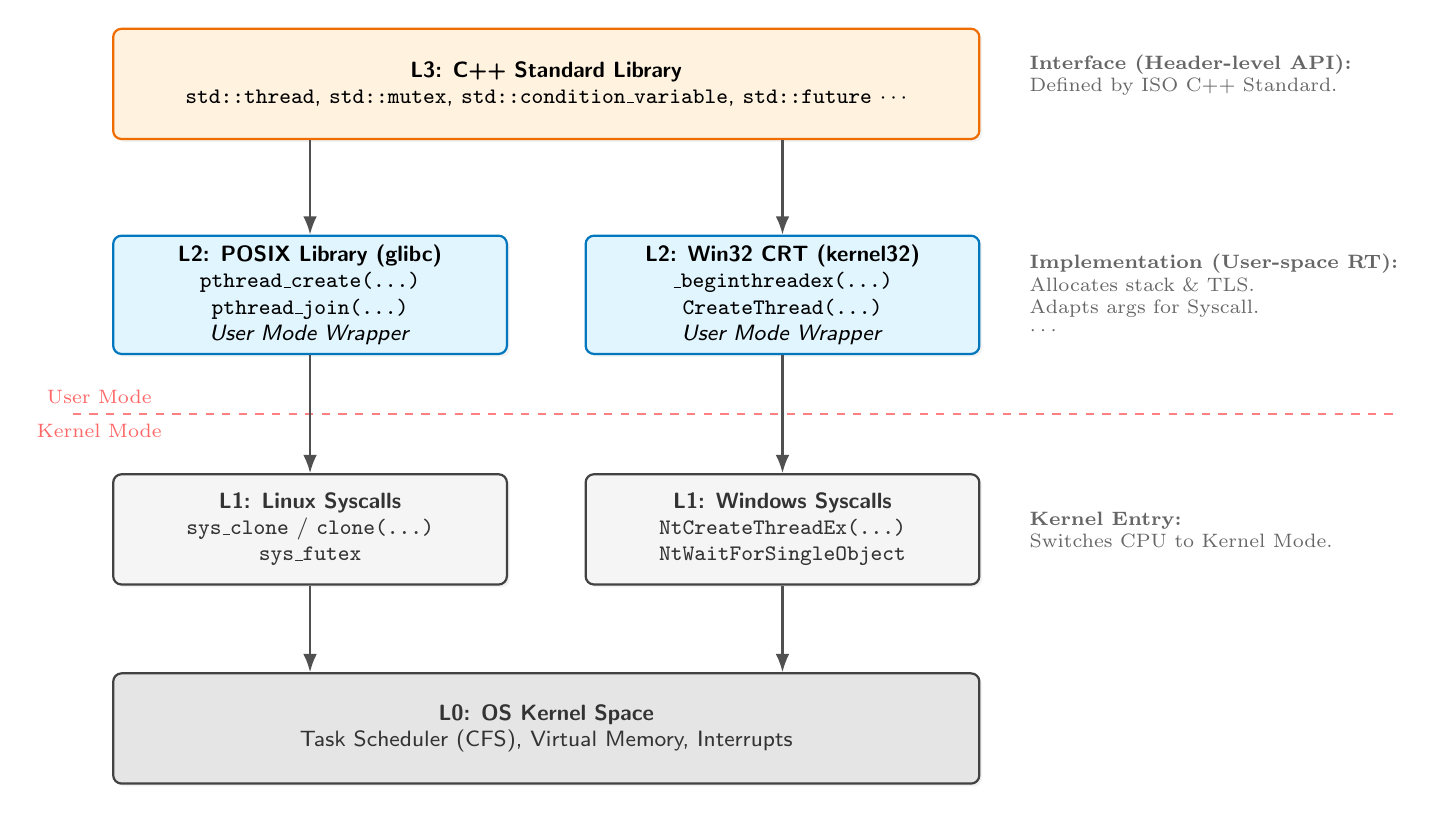
\begin{tikzpicture}[node distance=1.0cm]

	% ==========================================
	% 1. C++ 标准库层 (L3)
	% ==========================================
	\node [cppLayer, minimum width=11cm] (l5) {
		\textbf{L3: C++ Standard Library}\\
		\texttt{std::thread}, \texttt{std::mutex},
		\texttt{std::condition\_variable}, \texttt{std::future} $\cdots$
	};

	% --- 右侧注释 L3 ---
	\node [right=0.5cm of l5, noteText] (noteL3) {
		\textbf{Interface (Header-level API):}\\
		Defined by ISO C++ Standard.\\
	};

	% ==========================================
	% 2. 操作系统库层 (L2)
	% ==========================================
	% Linux (POSIX)
	\node [osLayer, below=1.2cm of l5.south west, anchor=north west, minimum width=5cm] (posix) {
		\textbf{L2: POSIX Library (glibc)}\\
		\texttt{pthread\_create(...)}\\
		\texttt{pthread\_join(...)}\\
		\textit{User Mode Wrapper}
	};

	% Windows (Win32)
	\node [osLayer, below=1.2cm of l5.south east, anchor=north east, minimum width=5cm] (win32) {
		\textbf{L2: Win32 CRT (kernel32)}\\
		\texttt{\_beginthreadex(...)}\\
		\texttt{CreateThread(...)}\\
		\textit{User Mode Wrapper}
	};

	% --- 右侧注释 L2 ---
	\node [noteText] at (noteL3.west |- posix) { % 对齐到 posix 节点
		\textbf{Implementation (User-space RT):}\\
		Allocates stack \& TLS.\\
		Adapts args for Syscall.\\
		$\cdots$
	};

	% ==========================================
	% 3. 系统调用层 (L1)
	% ==========================================
	% Linux Syscall
	\node [kernLayer, below=1.5cm of posix, minimum width=5cm] (sysLinux) {
		\textbf{L1: Linux Syscalls}\\
		\texttt{sys\_clone} / \texttt{clone(...)}\\
		\texttt{sys\_futex}
	};

	% Windows Syscall
	\node [kernLayer, below=1.5cm of win32, minimum width=5cm] (sysWin) {
		\textbf{L1: Windows Syscalls}\\
		\texttt{NtCreateThreadEx(...)}\\
		\texttt{NtWaitForSingleObject}
	};

	% --- 右侧注释 L1 ---
	\node [noteText] at (noteL3.west |- sysLinux) {
		\textbf{Kernel Entry:}\\
		Switches CPU to Kernel Mode.
	};

	% ==========================================
	% 虚线 (User vs Kernel Mode)
	% ==========================================
	\coordinate (boundaryY) at ($(posix.south)!0.5!(sysLinux.north)$);

	\draw [red!50, dashed, thick]
	($(sysLinux.west|-boundaryY) + (-0.5, 0)$) -- ($(noteL3.east|-boundaryY) + (0.5, 0)$)
	node [pos=0.02, above, text=red!60, font=\scriptsize] {User Mode}
	node [pos=0.02, below, text=red!60, font=\scriptsize] {Kernel Mode};

	% ==========================================
	% 4. 内核层 (L0)
	% ==========================================
	\node [kernLayer, below=0.5cm of sysLinux, minimum width=11cm, fill=black!10] (kernel)
	at ($(sysLinux.south)!0.5!(sysWin.south) - (0, 0.6)$) {
		\textbf{L0: OS Kernel Space}\\
		Task Scheduler (CFS), Virtual Memory, Interrupts
	};

	\draw [conn] (l5.south -| posix.north) -- (posix.north);
	\draw [conn] (l5.south -| win32.north) -- (win32.north);

	\draw [conn] (posix.south) -- (sysLinux.north);
	\draw [conn] (win32.south) -- (sysWin.north);

	\draw [conn] (sysLinux.south) -- (sysLinux.south |- kernel.north);
	\draw [conn] (sysWin.south) -- (sysWin.south |- kernel.north);

\end{tikzpicture}
\end{document}